% intro

Real-time Transport Protocol (RTP)~\cite{rfc3550} is suitable for multimedia
telephony (voice-over-IP, video conferencing, telepresence systems),
multimedia streaming (video-on-demand, live streaming), and multimedia
broadcast. RTP's design is based on the fundamental principles of \textit
{application-layer framing} and \textit{integrated layer
processing}~\cite{clark:alf}, i.e., it provides the following mechanisms:
source and payload type identification, packet playout time, stream
synchronization, packet loss and re-ordering, media stream monitoring. RTP
utilizes RTP Control Protocol (RTCP) to monitor the performance of the media
stream. Figure~\ref{fig:3:rtp:model} describes the features provided by RTP
and RTCP.

\begin{figure}[!h]
\centerline{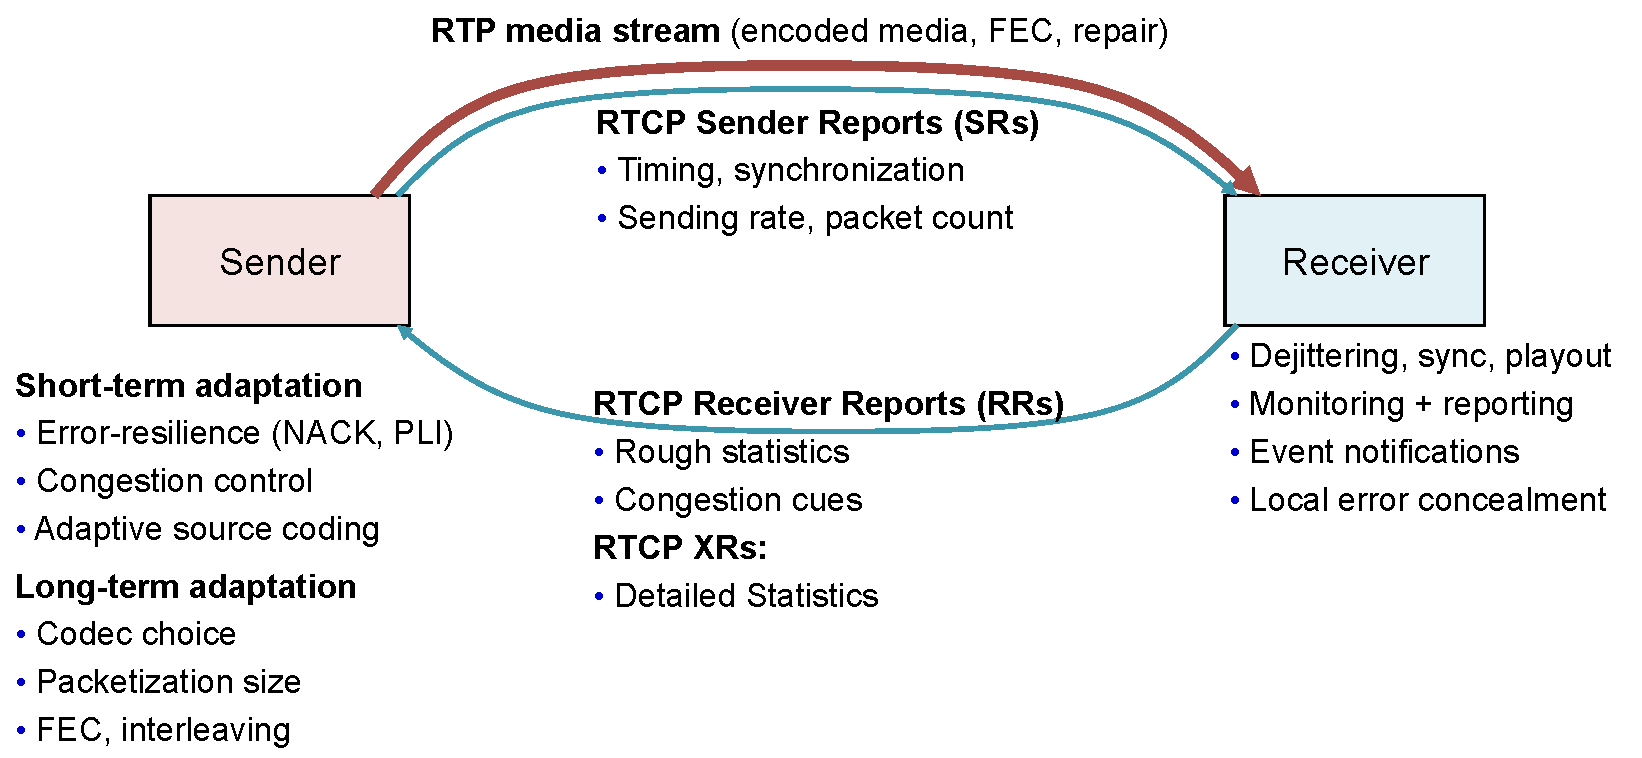
\includegraphics[width=\columnwidth]{chap3-rtp-rtcp}}
\caption{RTP and RTCP for adaptive real-time applications\\
{\scriptsize Source: J\"org Ott, ``Networked Multimedia Protocols and Systems''}}
\label{fig:3:rtp:model}
\end{figure}

Figure~\ref{fig:3:rtp.hdr} describes the RTP packet header format, the
\textit{`synchronisation source'} (SSRC) assists in determining the source
endpoint, typically useful when an endpoint sends multiple media streams that
need to be synchronized (e.g., Audio/Video lip-sync). The \textit{`RTP
timestamp'} assists in playing out the received packets at the appropriate
instance of time and recomposing the media frame from RTP packets. The
\textit{`RTP sequence number'} assists in identifying the lost packets and re-
ordering packets in case of out-of-order packet arrival. Lastly, RTP uses
\textit{`payload type'} (PT) to describe the encoding of the media data it is
carrying. Consequentely, each codec needs to specify its corresponding payload
format.

\begin{figure}[!h]
\centerline{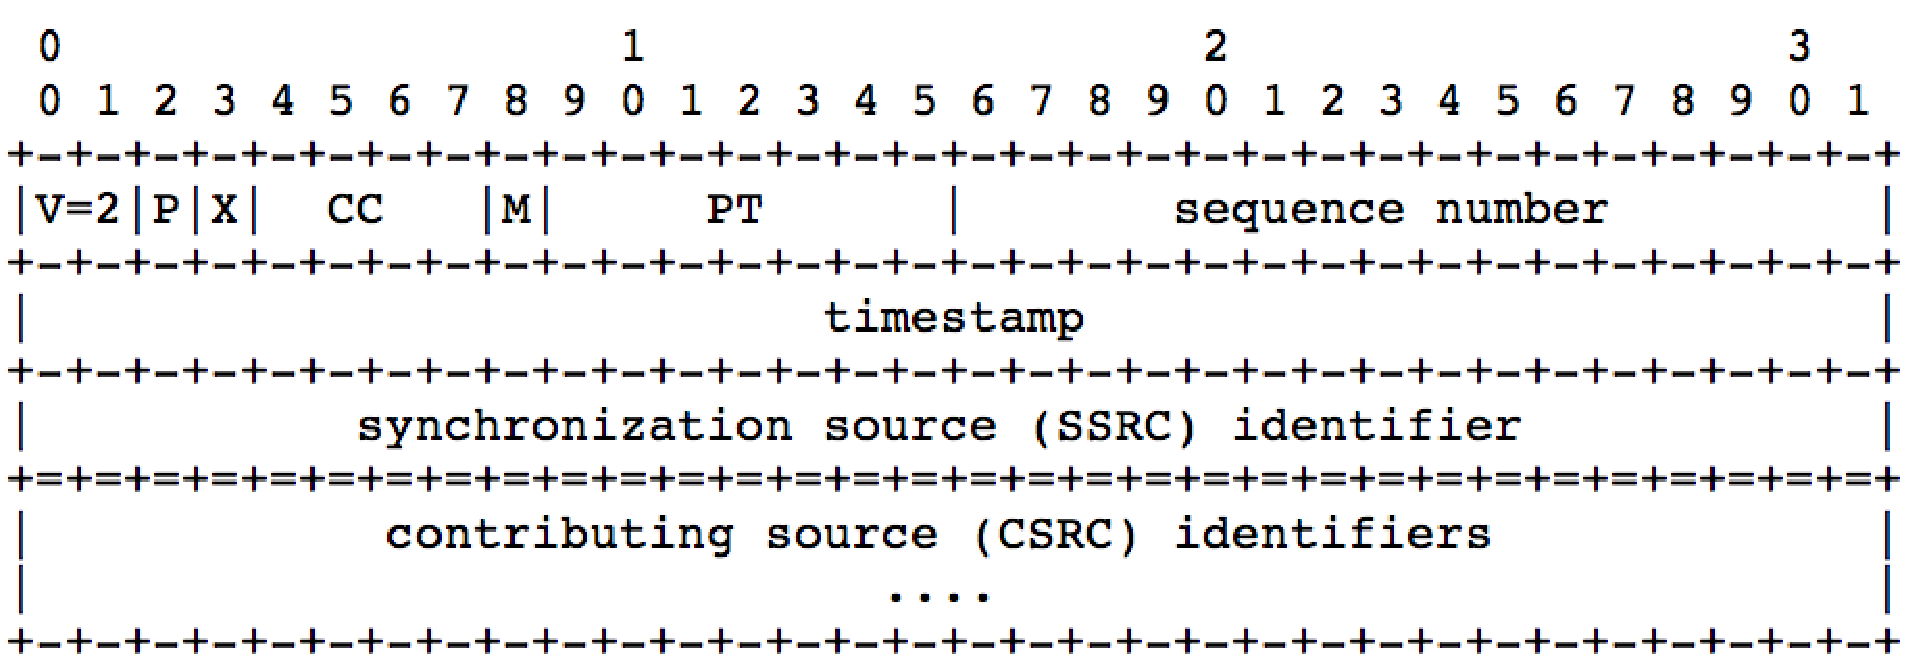
\includegraphics[width=\columnwidth]{fig_hdr_rtp}}
\caption{shows the RTP packet format that encapsulates the media data.}
\label{fig:3:rtp.hdr}
\end{figure}

\begin{figure}[!h]
\centering{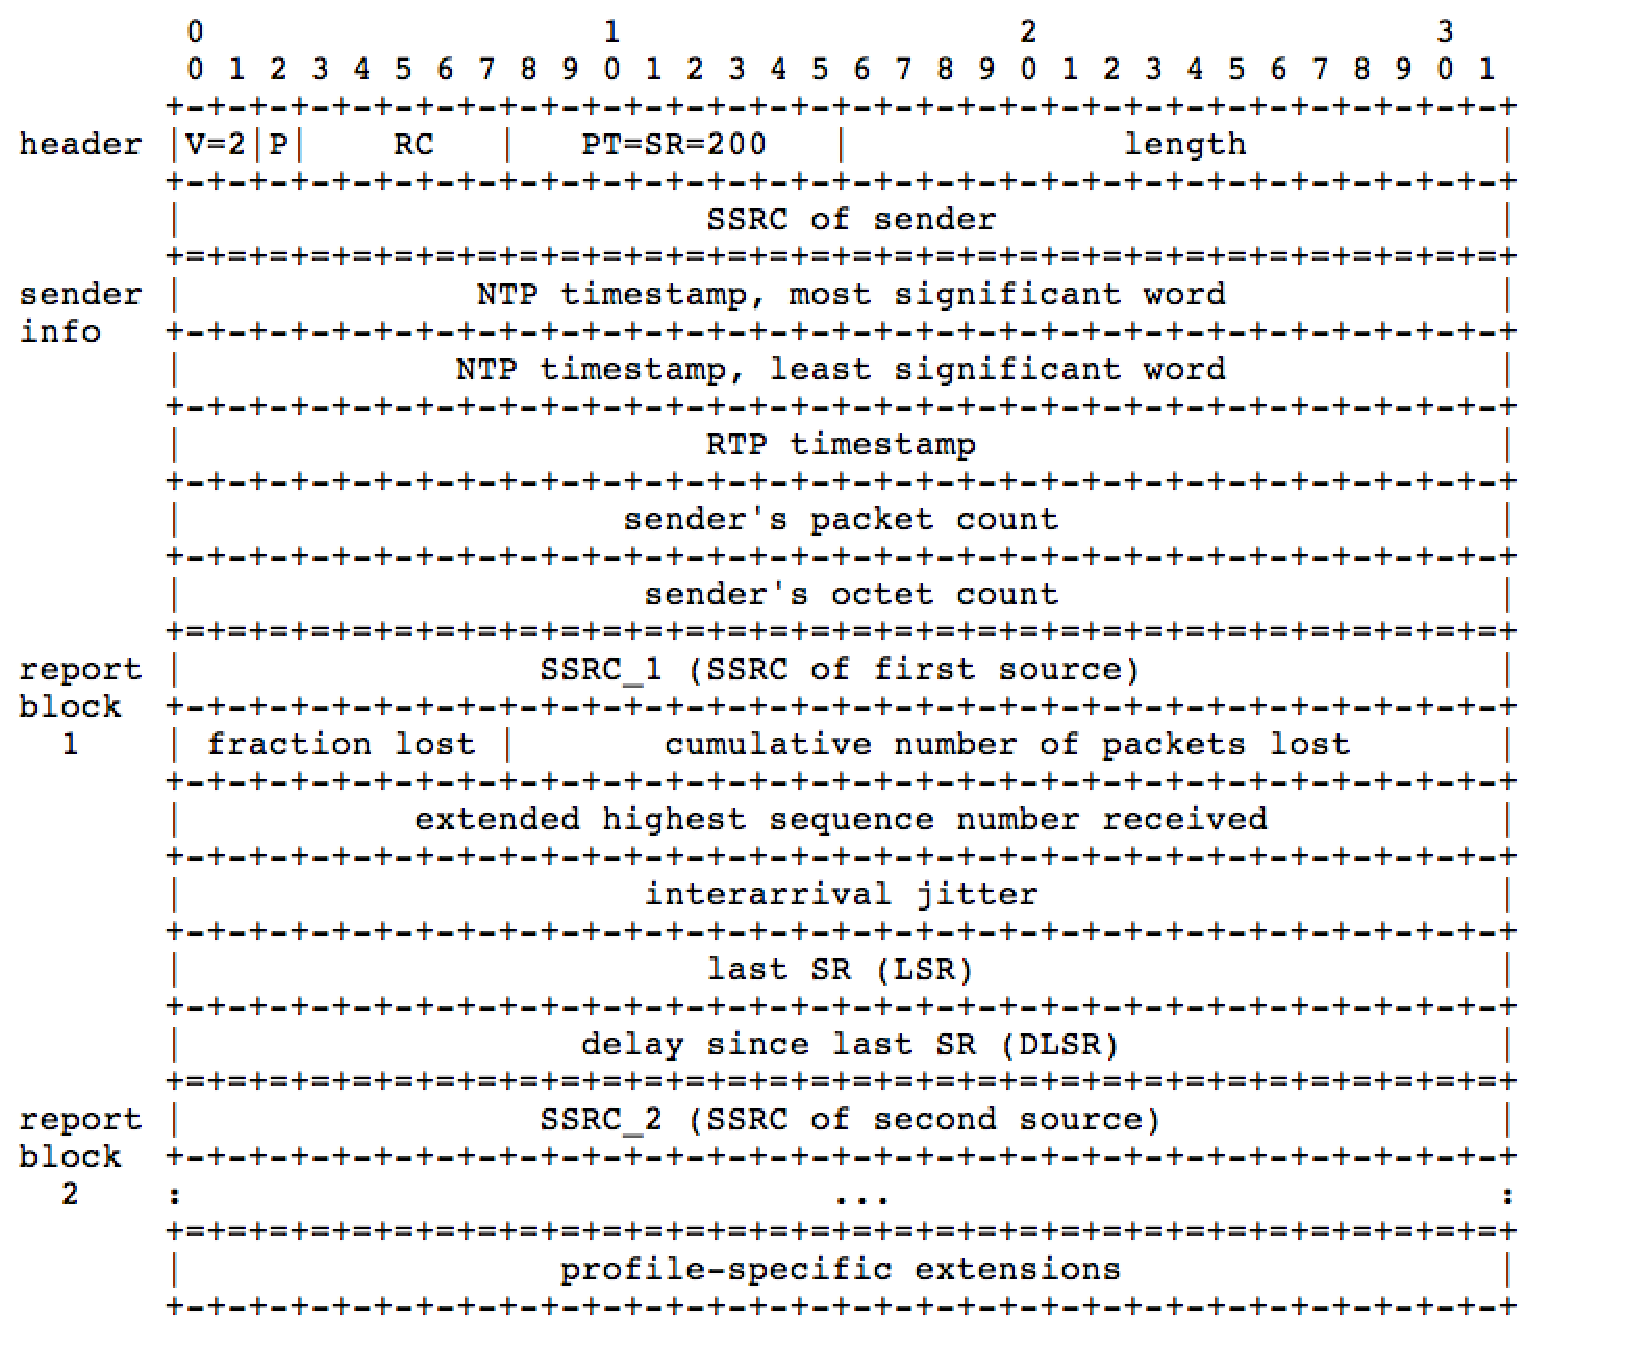
\includegraphics[width=\columnwidth]{fig_hdr_rtcp}}
\caption{shows the RTCP packet format for carrying the Sender Report (SR) and
the Receiver Report (RR). The SR carries transport statistics and enables 
stream synchronization, while the RR carries the receiver transport 
characteristics.}
\label{fig:3:rtcp.hdr}
\end{figure}

The receiver measures the incoming streams and reports the coarse-grained
transport statistics in an RTCP Receiver Report (RR). The RTCP RR contains the
current loss fraction, jitter, highest sequence number received, and
facilitates in calculating the RTT. The sender uses RTCP Sender Reports (SRs)
to assist in synchronizing the media streams (audio and video) by relating the
RTP timestamps of the individual media streams to the wall clock time (NTP)
and to notify the receiver about the current packet rate and bitrate.
Figure~\ref{fig:3:rtcp.hdr} describes the RTCP packet header format for a
interactive unicast media stream (i.e., both sending and receiving media).

\section{RTP Payload Formats}

The general principle for defining payload formats/types are to be able to
identify the encoding of the media packets. These encodings are either codec-%
specific (e.g., H.264, H.263, H.261, MPEG-1, MPEG-2, JPEG, G.711, G.722, AMR,
etc.), or generic (e.g., Forward Error Correction (FEC), Unequal Level of
Protection (ULP), NACK, multiplexed streams). Typically the payload format
specifies a well-defined packet format and packetization procedure. Hence, the
RTP header is immediately followed by payload-specific header (payload format)
and then by the media data. This allows the sending endpoint to enable
semantic-based fragmentation, which simplifies processing and decoding at the
receiver (i.e., be able to decode individual packets without relying on
receiving other packets).

\begin{figure}[!h]
\centerline{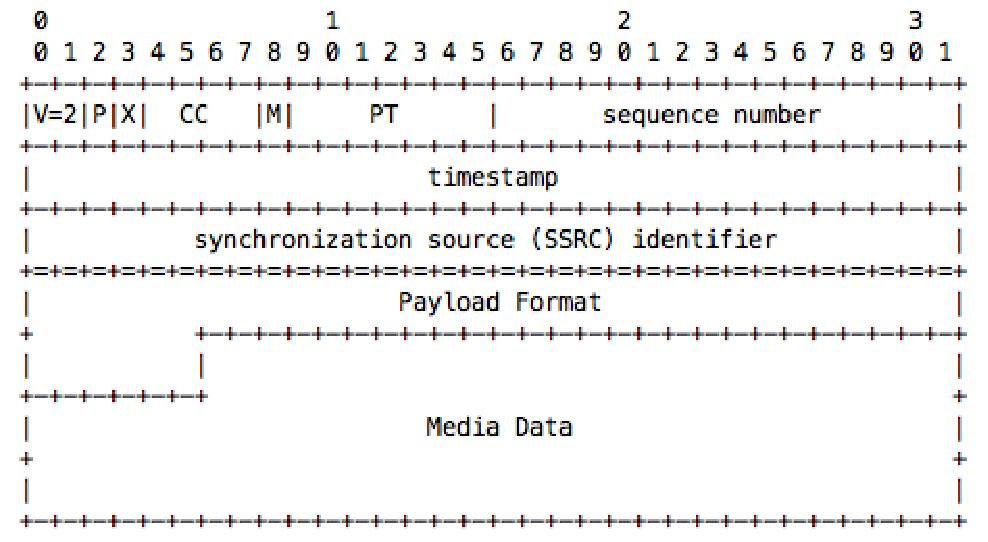
\includegraphics[width=\columnwidth]{fig_hdr_pt_fmt}}
\caption{shows the packet structure of an RTP packet encapsulating the
payload-specific header and the associated media data.}
\label{fig:3:pt.fmt}
\end{figure}

\section{RTP Header Extensions}

These extensions carry media-independent information, i.e., data that may be
repeated in multiple payload formats (e.g., timing information), and cannot be
reported in an RTCP report because RTCP is sent infrequently and unreliably.
The advantage of using header extensions is that they are 1) backwards
compatible, 2) can be ignored by an endpoint that does not understand them,
and 3) the sender is able to add multiple header extensions to an RTP packet.
Some current use-cases for RTP header extensions are: reporting the network
send timestamp (this allows the sender to pace large frames on to the network,
so not to cause temporary bandwidth overuse), client's audio levels (to
equalize audio levels across multiple streams in a video conference).

\section{RTCP Reporting Interval}
% timing

A closed control loop is formed by sending RTP media packets and receiving
RTCP feedback packets. The RTCP reporting interval is determined by the number
of SSRCs in the session, and the chosen session bandwidth. Typically, in a
unicast session there are two SSRCs, one for each participant, but the number
of SSRCs can be higher if each endpoint sends multiple media streams. The
interval between reports tends to be on the order of a few seconds, and is
randomized to avoid synchronization of reports from multiple endpoints.
Formally, to ensure that the RTCP reports are not sent too frequently, the
endpoints limit the feedback rate to $5\%$ of the session \textit{media rate},
shared equally by each participant in a video conference. Formally, the RTCP
reporting interval is calculated as follows:

\begin{align}
rtcp\_interval = & \frac{n \times avg\_rtcp\_size}{rtcp\_bw}
\label{eq:rtcp.int}
\end{align}
\hspace{35mm}$where,$
\begin{align*}
n &=  number\ of\ senders \\
rtcp\_bw &=  \frac{5}{100} \times media\_rate
\end{align*}


% avpf

If the endpoint detects packet loss or onset of congestion midway through a
reporting interval, the base RTP specification~\cite{rfc3550} (AVP profile)
does not allow sending the RTCP report early and the endpoint has to wait for
the next scheduled RTCP report. In this case, the slow control loop causes
instability and oscillation in the media bitrate. To overcome this
shortcoming, endpoints implement the Extended RTP Profile for RTCP-Based
Feedback (AVPF profile)~\cite{rfc4585}, an extension to RTP's default timing
rules to enable rapid feedback. This profile allows the endpoint to adjust the
RTCP reporting interval to send the RTCP feedback reports earlier than the
next scheduled RTCP report, sometimes even immediately. As long as reporting
interval on average remains the same. Figure~\ref{fig:3:avpf.interval} shows
the dynamics of the AVPF-enabled RTCP reporting interval.

\begin{figure}[!h]
\centerline{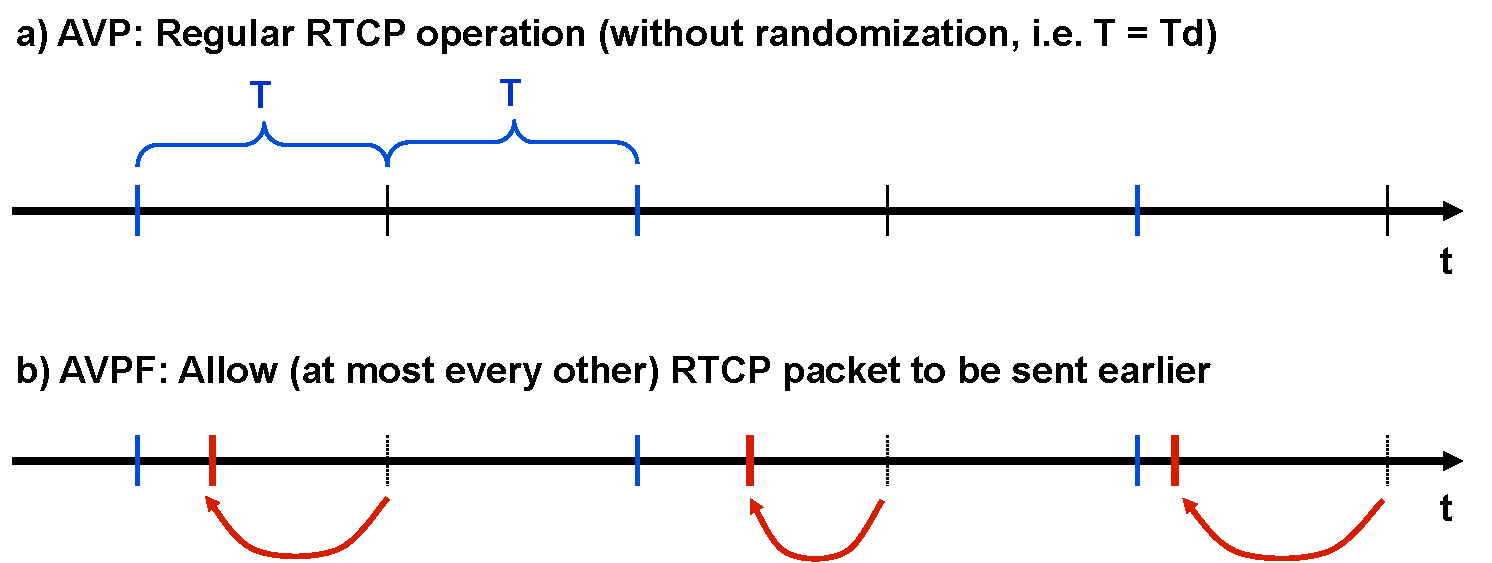
\includegraphics[width=\columnwidth]{chap3-avpf-rtcp}}
\caption{shows the RTCP reporting interval as defined in a) AVP, b) AVPF.}
\label{fig:3:avpf}
\end{figure}


Along with the possibility of providing timely feedback, the AVPF profile also
defines a suite of error-resilience feedback messages, namely, Negative
Acknowledgements (NACK), Picture Loss Indication (PLI), Slice Loss Indication
(SLI), Reference Picture Selection Indication (RPSI).

\section{RTCP Extended Reports (XRs) for Performance Monitoring}

Endpoints use RTCP XRs~\cite{rfc3611} to describe complex metrics that are not
exposed by the RTCP Receiver Report (RR). Some examples of XRs relevant to
performance monitoring and congestion control are: jitter buffer
metrics~\cite{draft.xr.jb}, Packet Delay Variation (PDV)~\cite{rfc6798},
summary statistics~\cite{draft.xr.stat}, delay metric~\cite{rfc6843}, burst-
gap discard/loss~\cite{rfc6958, draft.xr.bg.discard}, Run-Length Encoded (RLE)
loss/discard~\cite{draft.xr.discard.rle}, Quality of Experience
(QoE)~\cite{draft.xr.qoe}, and loss concealment~\cite{draft.xr.conceal}, etc.
RTP allows for new metrics to be defined, the only requirement is to document
what is measured, how it is measured and reported to the other endpoints.


% The RTCP Extended Reports (XR) [RFC3611] allow reporting of more
% complex and sophisticated reception quality metrics, but do not
% change the RTCP timing rules.  RTCP extended reports of potential
% interest for congestion control purposes are the extended packet
% loss, discard, and burst metrics [RFC3611],
% [I-D.ietf-xrblock-rtcp-xr-discard],
% [I-D.ietf-xrblock-rtcp-xr-discard-rle-metrics],
% [I-D.ietf-xrblock-rtcp-xr-burst-gap-discard],
% [I-D.ietf-xrblock-rtcp-xr-burst-gap-loss]; and the extended delay
% metrics [RFC6843], [RFC6798].


\section{Codec Control Messages}
% codec control

Sometimes an endpoint needs to configure or notify the other endpoint's codec.
These messages are broadly classified as \emph{Transport Layer} and  \emph
{Payload-specific} feedback messages~\cite{rfc5104}. The transport layer
messages are: Temporary Maximum Media Stream Bit Rate Request (TMMBR) and
Temporary Maximum Media Stream Bit Rate Notification (TMMBN). The receiving
endpoint uses the TMMBR message to configure the maximum encoding bitrate of
the media stream, while the sending endpoint uses the TMMBN to inform the
receiver of the updated bitrate. On the other hand, the payload-specific
messages are: Full Intra Request (FIR), temporal-spataial tradeoff, frame rate,
frame size, maximum packet size or packet rate, etc~\cite{draft.avt.cop}.

\section{Reduced-Size RTCP Reports}
% non-compound feedback

An endpoint sends RTCP feedback as a \emph{compound}, or \emph{minimal} RTCP
packet. A \emph{compound RTCP packet} is defined in~\cite{rfc3585}, contains
at least a sender report (SR) or a receiver report (RR) or both, followed by
Source Description (SDES) and any additional XR blocks. A \emph{minimal RTCP
packet} is one that contains a SR and/or RR, and followed by an SDES
containing just the canonical name (CNAME)\footnote{It is the real name
(identifier) used to describe the source, it can be in any form desired by the
user. Of the SDES items (username, email, phone, geo-location, etc.) CNAME is
compulsory to include in every RTCP packet.}. Hence, every compound RTCP
packet is a minimal RTCP packet with additional report blocks.

Consequently, including any of the additional SDES items or adding XR blocks
makes the compound RTCP packet very large. On a low bitrate links, during
transmission these large compound RTCP packets may introduce more delay.
Therefore, it may be desirable to logically fragment the report blocks in a
compound RTCP packet and send them independently. These fragmented report
blocks are called \emph{reduced-size RTCP packet}~\cite{rfc5506}. Unlike
compound RTCP packets, to transmit a reduced-size RTCP packet an endpoint does
not need to include the minimal RTCP report.

Reduced-size RTCP reports are beneficial in wireless networks where the packet
loss rate increases with the packet size, i.e., larger sized packets are more
likely to  be dropped compared to smaller sized packets. Additionally, smaller
packets have shorter serialization time, i.e., the amount of time it takes for
the endpoint to put the data packet on to the link.

The main reasons for the application to use the reduced-size RTCP reports are:
1) notify the other endpoint of events, using the signaling channel would
incur at least one RTT while implementing it as an RTCP extension would merely
incur a one-way delay. 2) send codec control (e.g., TMMBR) or feedback (e.g.,
NACK, RPSI) messages, these messages as reduced-size are more likely to be
transmitted compared to the compound packets and with as little delay as
possible. Especially since these types of messages are more likely to be sent
when link conditions are poor.


% relationship with SDP
\section{Session Setup}

% SDP O/A, declarative SDP, RTCP notify

There are several ways to setup an interactive or conversational multimedia
session, for example by implementing one of the following:
H.323~\cite{H.323}, Session Initiation Protocol (SIP)~\cite{rfc3261},
Jingle~\cite{XEP-0166} an extension to Extensible Messaging and Presence
Protocol (XMPP)~\cite{rfc6120}. 

SIP uses Session Description Protocol (SDP)~\cite{rfc4566} to describe the
endpoint's transport and media capabilities. An SDP description defines only
one multimedia session, i.e., an association between a set of participants.

\begin{figure}[!h]
\centerline{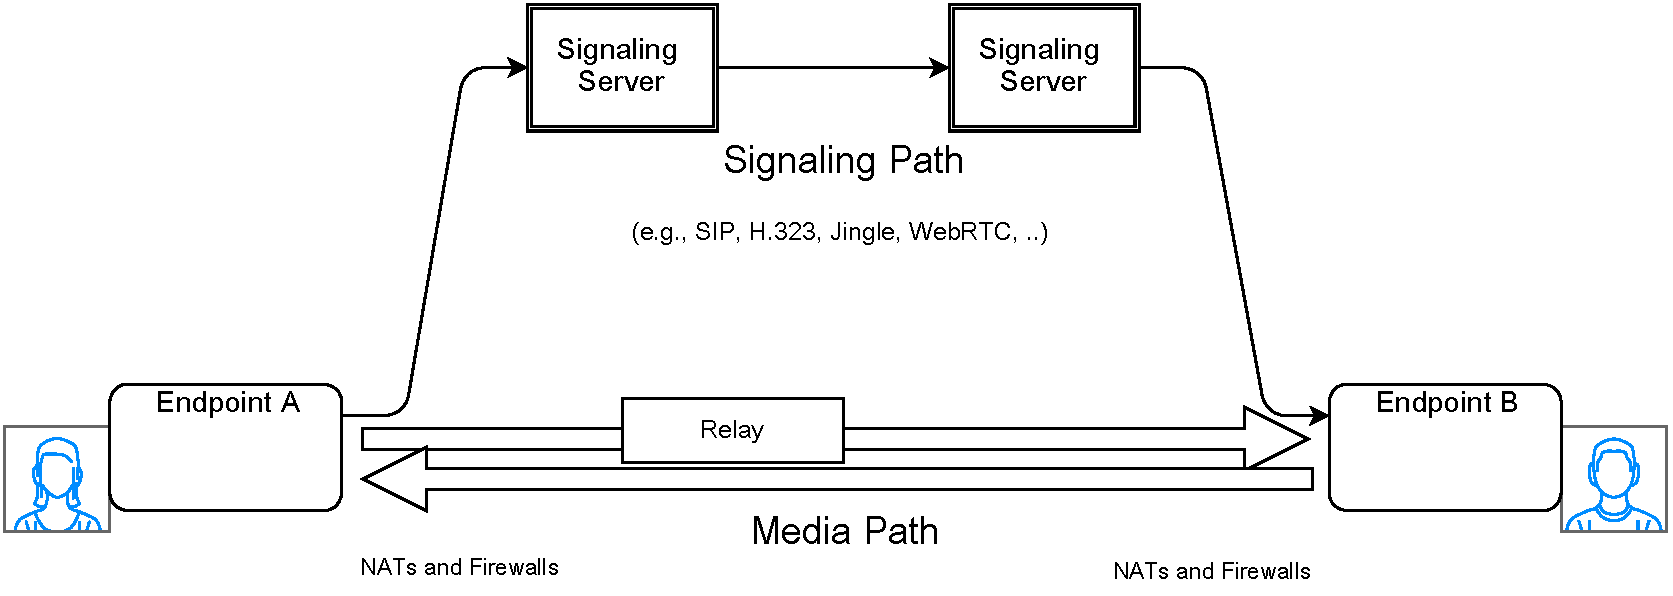
\includegraphics[width=\columnwidth]{chap3-sig-med}}
\caption{shows the signaling and media paths between two endpoints engaging in
a video call.}
\label{fig:3:sig.media}
\end{figure}


The transport details in the SDP are mainly split into two parts: the protocol
for delivering media packets (currently, TCP, UDP, or SCTP) and the outgoing
IP address of the endpoint. The protocol to deliver the media packets is
chosen by the application, but identifying the outgoing IP address of an
endpoint is a bit complex. This is due to the presence of NAT devices in the
network, which may change the IP address of the outgoing packets. Since,
interactive media calls are between endpoints and media streams may have to
traverse through a NAT at both ends, in some cases, the only way to deliver
media packets between the two endpoints would be by accessing a relay on the
public Internet. Hence, the endpoint needs to discover its 2-tuple [IP
address:port] on the host, NAT~\cite{rfc5389} and the allocated
relay~\cite{rfc5766} before it notifies the other endpoints about its
transport details. This collection of 2-tuples is known as \emph{candidates}
and both endpoints exchange their candidate addresses in the SDP. On receiving
the candidates, the endpoint performs a probe between each combination of
addresses in the two candidate lists and chooses the first one that is
successfully received (\emph{aggressive nomination}). This process of
performing pair-wise \emph{connectivity checks} is called Interactive
Connectivity Establishment (ICE)~\cite{rfc5245, rfc6544} and it relies on
\emph{Session Traversal Utilities for NAT} (STUN) protocol to establish
connectivity across a NAT and in case it fails to establish connectivity, it
uses \emph{Traversal Using Relays around NAT} (TURN) protocol to use a relay
on the public Internet to deliver the media packets.

% Depending on the type of NAT device (full-cone, address- or port-restricted
% cone, symmetric).

\begin{figure}[!h]
{\small
\begin{verbatim}
        v=0
        o=jdoe 2890844526 2890842807 IN IP4 10.0.1.1
        s=
        c=IN IP4 192.0.2.3
        t=0 0
        a=ice-pwd:asd88fgpdd777uzjYhagZg
        a=ice-ufrag:8hhY
        m=audio 45664 RTP/AVP 0
        a=rtpmap:0 PCMU/8000
        a=candidate:1 1 UDP 2130706431 10.0.1.1 8998 typ host
        a=candidate:2 1 UDP 1694498815 195.148.127.98 45664 typ srflx 
            raddr 10.0.1.1 rport 8998
\end{verbatim}
}
\caption{Sample SDP containing the sender's transport and media capabilities.}
\label{fig:3:sdp}
\end{figure}

The second part of SDP carries the media capabilities, which binds the SDP to
the Offer/Answer (O/A) model. In the O/A model, the sending endpoint sends to
the receiver a set of media capabilities (\emph{offer}) in decreasing order of
preference, typically, multiple options of audio codecs and video codecs. On
receiving the sender's capabilities, the receiver compares its media
capabilities with the sender's and responds with the one that best fits the
receiver's requirements (\emph{answer}). The \emph{offer is rejected} in the
case where the receiver is unable to pick any of the options provided by the
sender. Hence, the application at the sender needs to pick a minimum number of
widely available audio and video codecs to avoid negotiation failure. If the
\emph{offer is accepted}, both endpoints then know the following: 1) which
audio and/or video codecs to use, 2) the payload type of the encoded media
streams (possibly even their respective SSRCs), 3) to which IP address and
port number to send the media stream, 4) the media session bandwidth and 5)
encryption keys for encrypting traffic.
